\chapter{Tecnologie utilizzate}
\label{cha:tecnologie_utilizzate}

La prima parte del tirocinio è stata investita per comprendere come implementare la mia idea all'interno del progetto DISI Industry, dunque è stato necessario comprendere le tecnologie utilizzate per lo sviluppo di quest'ultimo per permettere lo sviluppo del mio applicativo all'interno di esso, mantenendo una continuità e coerenza con il resto della piattaforma, sia a lato front-end che a lato back-end.

In questo capitolo vengono presentate le tecnologie utilizzate e le motivazioni dietro tali scelte. In particolare, vengono presentate le tecnologie utilizzate per la realizzazione del back-end, del front-end e del database.

\section{Django}
Il framework utilizzato è Django, esso è stato scelto per la sua semplicità di utilizzo e per la sua flessibilità. Django è un framework open-source di alto-livello per lo sviluppo di applicazioni web scritto in Python e permette lo sviluppo di webapp funzionali e sicure senza il bisogno di utilizzare plugin esterni per avere funzionalità che possono essere considerate necessarie per una webapp moderna, in quanto si occupa dal'accesso ai dati del database al routing all'interno della webapp. Esso è basato sul pattern architetturale Model-View-Template (MVT) e permette di sviluppare applicazioni web in modo rapido e pulito, fornendo un'interfaccia di amministrazione per la gestione dei dati, così da non dover implementare un'area per l'amministratore mediante un altro linguaggio o estensioni esterne, ma mantenendo unificata la codebase.

Un altro vantaggio risiede nella scalabilità del framework, il quale permette la creazione di moduli che possono essere inseriti o rimossi con l'aggiunta di poche righe di codice all'interno di un file apposito.


Data la natura del progetto, è stato necessario avere un framework che permettesse la creazione, validazione e modifica dei form, difatti Django offre un componente apposito per la gestione dinamica dei form dalle View, senza dover passare per il codice html evitando dunque non solo inconsistenza in tutta la codebase, ma anche assicurando un livello maggiore di mantenibilità di codice, in quanto tutti i form sono in un'area specifica. Per la visualizzazione dei form dinamicamente e con dello stile unificato viene utilizzato il modulo Crispy Forms per permettere di controllare come il form venga renderizzato dall'utente finale. \cite{crispy_forms}


\subsection{Architettura MVT}
Il vantaggio dell'utilizzo di un framework basato su architettura MVT permette ad ogni livello, ossia Model, View e Template, di lavorare indimendentemente, il che comporta una maggiore indipendenza tra le parti. Esso è conveniente nel caso si decida di scalare l'applicativo web, in quanto permette di aggiungere nuove funzionalità senza dover modificare il codice già esistente. Inoltre, un'architettura MVT permette di rendere più veloce e più seplice la trasmissione di dati via internet data la natura ed il funzionamento dell'architettua stessa.


Vengono presentati in dettaglio le componenti dell'architettura MVT:
\begin{itemize}
    \item Model : questo componente aiuta la gestione del database ed esso è un livello di accesso dati che contiene i campi ed il comportamento dei dati che stanno venendo gestiti. Esso utilizza un pattern ORM (Object-Relational Mapping) che mappa i campi del database con gli attributi della classe Python. Questo permette di utilizzare un linguaggio di programmazione orientato agli oggetti come Python per la gestione dei dati, permette un livello di astrazione tale da non rendere obbligatoria la stesura di query in linguaggio SQL, inoltre permette una maggiore semplicità durante la manutenzione del codice dovuta al fatto che solamente un linguaggio viene utilizzato. Mediante ORM è anche possibile cambiare database in modo efficace ed efficiente, in quanto non è necessario apportare modifiche al codice già esistente che detiene la struttura dei modelli del Database.
        I modelli aiutano  ad effettuare le operazioni CRUD (Create, Read, Update, Delete) sul database in modo semplice e veloce. Inoltre, Django permette di definire delle relazioni tra i modelli, in modo da poter accedere ai dati in maniera semplice e veloce, oltre alla definizione di ciò che viene definita Business Logic del programma (es. validazione dei dati, ecc.). \cite{django_models}
\item View : Esso può essere visto come l'organo esecutivo della Business Logic, in quanto permette di interagire con i modelli definiti dal modulo Model e  gestisce la renderizzazione in template. La view ottiene i dati dal Model, dopodichè può modificare i suddetti ed eventualmente renderizzarli in un template. Esso accetta richeste HTTP(HyperText Transfer Protocol), applica la business logic e fornisce risposte HTTP al client. \cite{django_views}
    \item Template : Questo modulo è il livello più vicino all'utente, in quanto è un livello di presentazione che gestisce completamente l'interfaccia dell'utente. Esso viene rappresentato mediante file con codice HTML(HyperText Markup Language) che vengono utilizzati per renderizzare dati ed essi possono contenere dati statici o dinamici. Nel caso di Django viene utilizzato un lingaggio speciale chiamato Django Template, il quale permette la definizione di variabili, cicli, condizioni, ecc. oltre ai comandi classici di HTML, per rendere più semplice e leggibile il codice. Esso, inoltre, permette di definire un template base, il quale può essere esteso da altri template. \cite{django_template}
\end{itemize}


Di seguito viene rappresentato un diagramma esplicativo dell'architettura del Framework Django.

\begin{figure}[H]
    \centering
    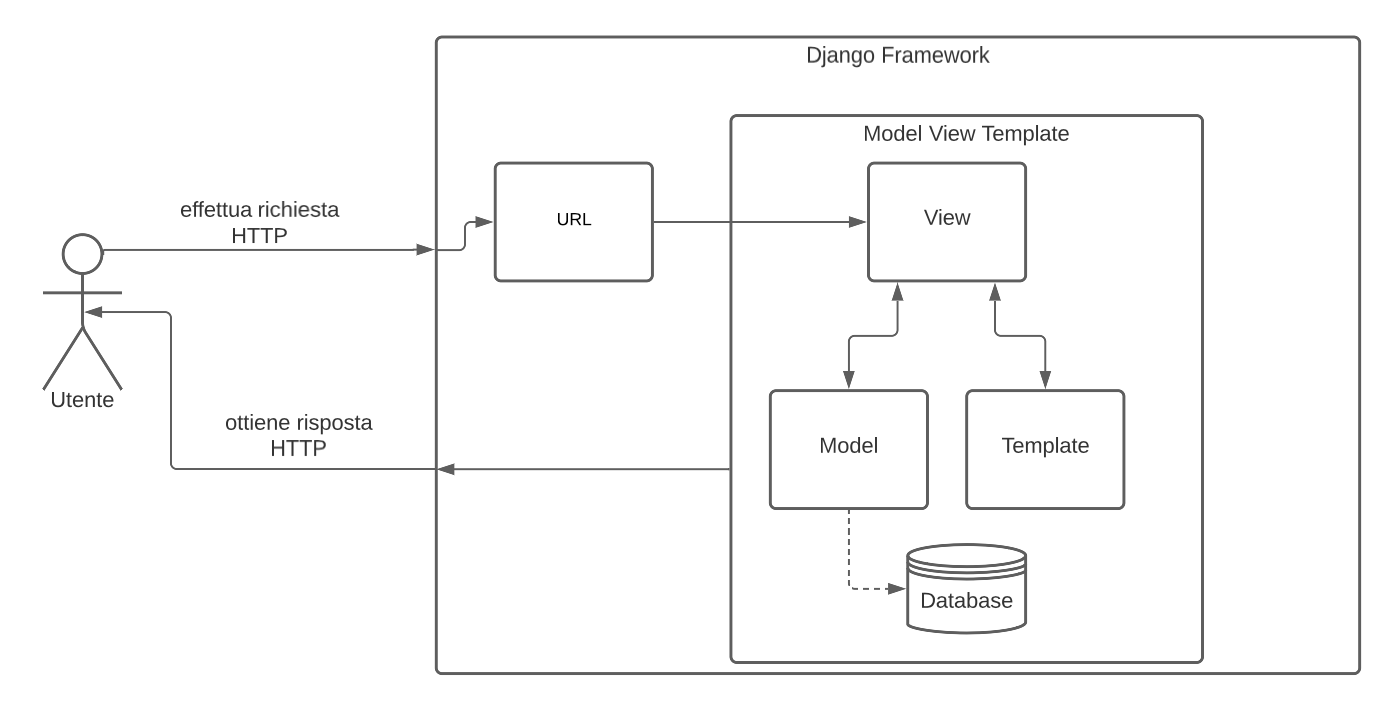
\includegraphics[scale=0.42]{images/architettura_django.png}
    \caption{Architettura del framework Django}
    \label{img:architettura_django}

\end{figure}

Il processo di una richiesta e risposta HTTP utilizzando il framework Django è il seguente:
\begin{enumerate}
    \item L'utente interagisce mediante il proprio browser con il front-end dell'applicativo.
    \item L'utente effettua una richiesta HTTP dal browser fornendo un URL(Uniform Resource Locator). 
    \item Django valuta l'URL e controlla che esista una View corrispondente a tale URL. 
    \item Entrando nel Model View Template la View cattura la richiesta, elabora i dati ed invia una risposta. Possono accadere le seguenti azioni :
    \begin{enumerate}
        \item La View richiede l'accesso a dei dati al componente Model : la query espressa sottoforma di linguaggio python viene valutata e trascritta nel linguaggio del database (nel contesto di questo specifico applicativo in SQL) e fornisce il QuerySet(l'insieme dei dati richiesti) alla View.
        \item Con i dati ottenuti la view effettua delle modifiche a questi dati ed invia una copia al componente Model. 
        \item Se richiesto, utilizzando i dati ottenuti, la view formula una richiesta di visualizzazione di una pagina HTML al componente Template e passa come argomenti gli eventuali dati aggiuntivi ottenuti. Una volta ricevuta la richiesta tale modulo genera i dati HTML necessari e li restituisce alla View
    \end{enumerate}
    \item Dopo aver fornito una risposta a Django, il componente View si incarica dell'inviare la risposta HTTP della richiesta effettuata mediante URL.
    \item Il front-end cattura la risposta ed il browser predefinito dell'utente renderizza la risposta per permettere la visualizzazione.
\end{enumerate}

Ovviamente nel caso l'operazione del CRUD pattern sia una Create o una Delete e non una Read o Update, la richiesta di accesso ai dati del Database da parte del componente View sarà gestita in maniera appropriata(fornire l'accesso al dato e salvare l'entry nel database nel caso di una Create, o fornire la possibilità di eliminare una specifica entry nel database nel caso di una Delete).
\subsection{Sicurezza}

Un altro vantaggio del framework Django è la sicurezza, in quanto nativamente supporta dei controlli che possono essere facilmente inclusi sfruttando il livello d'astrazione fornito da un framework. \cite{django_security}

Oltre ai controlli sull'autenticazione, autorizzazione e gestione delle sessioni, tale framework permette di evitare attacchi tra i quali:
\begin{itemize}
    \item SQL Injection : Attacco volto all'inserimento di codice SQL in input non controllati, in modo da poter accedere ai dati del database. Django permette di evitare tale attacco in quanto permette di utilizzare un linguaggio di programmazione orientato agli oggetti come Python per la gestione dei dati, applicando ciò che viene definito \textit{input sanitizing}, il quale permette di evitare l'inserimento di codice SQL in input non controllati.
    \item Cross Site Scripting(XSS) : Tale attacco permette all'utente di inserire codice HTML e JavaScript malevolo che verrà poi visualizzato dagli altri utenti dell'applicazione mediante la pressione di un link o bottone. Tale problema viene risolto mediante input sanitizing e l'escape automatico di caratteri non sicuri.
    \item Cross Site Request Forgery(CSRF): L'attacco CSRF sfrutta il fatto che molte applicazioni web autenticano gli utenti utilizzando sessioni o token di autenticazione, ma non validano in modo appropriato la fonte delle richieste che vengono inviate. In un attacco CSRF, un malintenzionato crea una pagina web malevola o un messaggio e lo fa visualizzare all'utente target mentre è autenticato in un'altra applicazione web.

Quando l'utente visualizza questa pagina o questo messaggio, il codice maligno presente al suo interno genera una richiesta HTTP verso l'applicazione web bersaglio, sfruttando la sessione o il token di autenticazione dell'utente. Poiché l'applicazione web bersaglio considera la richiesta legittima, esegue l'azione richiesta, che potrebbe essere, ad esempio, un trasferimento di fondi, una modifica delle impostazioni dell'account o l'invio di un messaggio. Django permette di evitare tale attacco mediante l'utilizzo di un token di sicurezza.

    \item Clickjacking : Attacco che mira ad ingannare l'utente mediante il click di zone nascoste o trasparenti. Django permette di evitare tale attacco mediante l'utilizzo di un middleware che permette di inserire un'intestazione HTTP.

\end{itemize}

\subsection{Virtual Environment}
Per assicurarsi della totale compatibilità tra DISI Industry e l'applicativo sviluppato, è stato utilizzato un virtual environment, ovvero un ambiente virtuale che permette di isolare le dipendenze di un progetto Python installando i pacchetti in una directory specifica anziché in tutto il sistema. Il virtual environment utilizzato è stato \textit{venv} \cite{venv} e la versione di python utilizzata è python 3.8.



\section{Front-end}
In questa sezione vengono riportate le tecnologie utilizzate per permettere lo sviluppo dell'interfaccia front-end dell'applicativo. Tali teconologie sono state utilizzate per assicurarsi di ottenere una webapp che sia in primo luogo responsive, ossia che si adatti dinamicamente a diversi dispositivi, mentre in secondo luogo che sia user-friendly e con un'interfaccia semplice ed intuitiva.

Nel capitolo \ref{cha:front-end} vengono presentati degli screenshot e viene descritta velocemente l'interfaccia dell'applicativo.
\subsection{Bootstrap}
Per poter implementare blocchi di stile in modo efficiente e per rendere l'applicazione responsive viene utilizzato Bootstrap, un framework open-source di sviluppo Front-end e viene considerato il framework CSS più utilizzato per creare applicativi web e Mobile-first.

Tale framework è estremamente personalizzabile, è compatibile con tutti i browser moderni e permette di evitare inconsistenze nel caso vengano utilizzati browser differenti.
Precisamente viene utilizzato Bootstrap v5.0 \cite{bootstrap}

\subsection{SCSS}
Per permettere la customizzazione di alcuni elementi di stile, viene utilizzato Sassy Cascading Style Sheets (SCSS), una delle estrensioni del classico CSS più stabili, mature e potenti che permette di utilizzare variabili, annidamento, mixin, import, ereditarietà e altro, rendendo più semplice la scrittura di codice CSS. \cite{scss}

\section{Autenticazione ed Autorizzazione}
Seguendo il principio \textit{Separation of concerns}, l'autenticazione e l'autorizzazione vengono gestite da due componenti differenti, in modo da permettere una maggiore manutenibilità e scalabilità del sistema.
Per permettere agli utenti di accedere alle risorse controllando che la loro identità corrisponda con quanto loro abbiano dichiarato, viene utilizzato Shibboleth per il processo di autenticazione. Per quanto concerne l'autorizzazione, invece, vengono utilizzate funzioni interne di Django e viene utilizzato un sistema di permessi basati su ruoli, i quali vengono assegnati agli utenti in base al loro ruolo all'interno dell'applicazione, seguendo quindi un modello RBAC - Role Based Access Control.



\section{Shibboleth}
Viene di seguito presentato il software di autenticazione utilizzato. 


Esso è un framework open-source per l'autenticazione federata e l'autorizzazione basata su attributi, utilizzato da molte organizzazioni e istituzioni per fornire l'accesso a risorse web protette. Esso è una implementazione di SAML - Security Assertion Markup Language e ciò permette al software di operare come SSO - Single Sign On. \cite{shibboleth}

Di seguito viene riportato un Sequence Diagram semplificato che mostra il processo di autenticazione di Shibboleth. Bisogna notare che valgono le seguenti assunzioni :
\begin{itemize}
    \item L'utente non ha già effettuato l'accesso al suo Identity Provider.
    \item Le credenziali inserite dall'utente sono valide.
    \item La risorsa richiesta è presente nel sistema e la richiesta di accesso alla risorsa è correttamente formata (il che significa che l'URL fornito è valido)
    \item L'utente ha le corrette capacità per accedere alla risorsa richiesta.
    \item Il Service Provider è l'applicazione web.
    \item L'Identity Provider è l'IdP dell'Università degli Studi di Trento.
\end{itemize}
\newpage


\begin{figure}[H]
    \begin{center}
        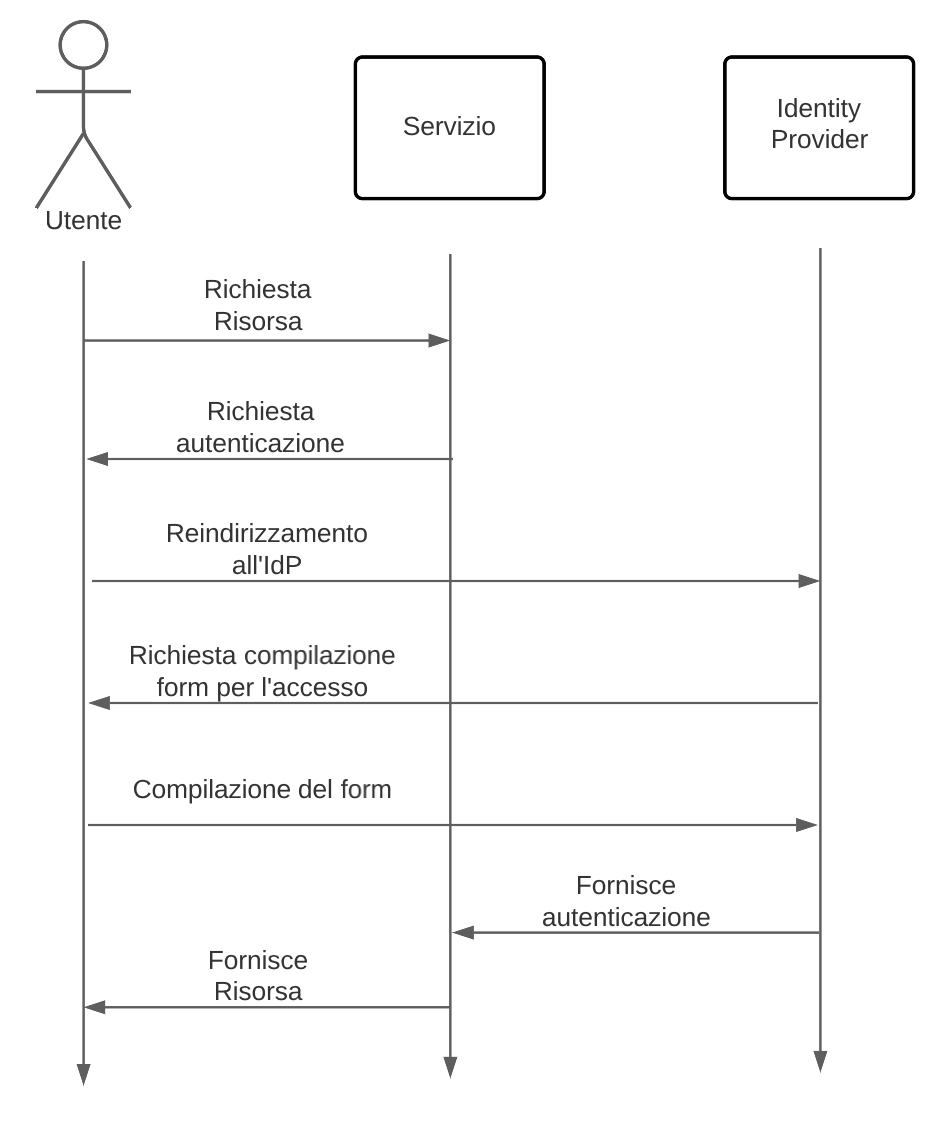
\includegraphics[width=0.65\textwidth]{images/shibboleth_auth.png}
    \end{center}
    \caption{Processo di autenticazione di Shibboleth}
    \label{fig:shibboleth_auth}
\end{figure}


Descrizione del processo di autenticazione di Shibboleth:
\begin{enumerate}
    \item L'utente richiede l'accesso ad una risorsa protetta.
    \item Il Service Provider che detiene la risorsa, in questo caso l'applicativo web, genera un messaggio SAML e redireziona l'utente al suo Identity Provider.
    \item L'Identity Provider cattura il messaggio SAML e richiede all'utente di autenticarsi mediante un form apposito.
    \item L'utente inserisce le sue credenziali ed il form viene inviato all'Identity Provider.
    \item L'Identity Provider genera una sessione e controlla la Attribute Release Policy per definire quali attributi vengono forniti all'utente, dopodichè genera un messaggio SAML contenente i dati dell'utente e lo invia al Service Provider.
    \item Il Service Provider cattura il messaggio SAML e controlla la firma digitale per verificarne l'autenticità.
    \item Il Service Provider fornisce la risorsa richiesta dall'utente.
\end{enumerate}
\section{Mail}
Per l'invio di email agli utenti quando richiesto dal sistema, viene utilizzato un mail server che implementa il protocollo SMTP - Single Mail Transfer Protocol. Tale server è configurato come relay ad un altro mail server interno all'università ed è quest'ultimo che si occupa di inviare effettivamente le email agli utenti.

La configurazione Relay permette al server al quale vengono passate le richieste di invio mail da parte di Django di inoltrarle al server interno all'università, che si occuperà di inviare le email agli utenti. Questa configurazione è stata necessaria in quanto il server interno all'università non è raggiungibile dall'esterno e tale scelta è stata effettuata per assicurare flessibilià, scalabilità e sicurezza al sistema.


\clearpage
